% !TEX program = lualatex
% MHM2010 Correction Workbench documentation
% Version: 0.2.2 | Author: William W. Wallace | Created: 2026-11-03 | Modified: 2026-11-05
% Revision: 0.1.0 Initial operator manual, validation and equation appendix.
%           0.2.0 T4 iMaser 3000, reference 1 PPS figures, MJD/local time axes.
%           0.2.1 T4 monitoring files (FTP ./Monitoring), operator reboot
%                 script, local UDP port 14000, REBOOT wording and page cites.
%           0.2.2 View > Time display (MJD / ISO 8601 local / UTC), fit
%                 windows (last 30 and 90 days), where the Veusz files are.
% Build twice: lualatex -interaction=nonstopmode -halt-on-error <this file>
\documentclass[11pt,a4paper]{article}
\usepackage[margin=19mm,headheight=16pt]{geometry}
\usepackage{fontspec}
\setmainfont{TeX Gyre Pagella}
\setsansfont{TeX Gyre Heros}
\setmonofont{Latin Modern Mono}[Scale=0.88]
\usepackage{amsmath,amssymb,booktabs,longtable,array,graphicx,xcolor}
\usepackage{enumitem,fancyhdr,listings,xurl}
\usepackage[unicode,colorlinks=true,linkcolor=teal,urlcolor=teal,
  bookmarksopen=true,bookmarksnumbered=false,pdfpagelabels=true]{hyperref}
\usepackage{bookmark}
\definecolor{navy}{HTML}{172C40}
\definecolor{teal}{HTML}{176B79}
\definecolor{light}{HTML}{EFF5F7}
\setcounter{secnumdepth}{0}
\setcounter{tocdepth}{1}
\setlength{\emergencystretch}{2em}
\setlength{\parindent}{0pt}
\setlength{\parskip}{6pt}
\setlist[itemize]{leftmargin=5mm,itemsep=3pt,topsep=3pt}
\pagestyle{fancy}
\fancyhf{}
\fancyhead[L]{\sffamily\small MHM2010 / T4 MASER TIMING WORKBENCH}
\fancyhead[R]{\sffamily\small 0.2.2}
\fancyfoot[L]{\sffamily\footnotesize Engineering analysis; no maser writes}
\fancyfoot[R]{\sffamily\footnotesize\thepage}
\renewcommand{\headrulewidth}{0.4pt}
\hypersetup{pdftitle={MHM2010 / T4 Maser Timing Workbench: Operator and Scientific Manual},
 pdfauthor={William W. Wallace},pdfsubject={Version 0.2.2, Python 3.12, MHM2010 and T4 iMaser 3000}}
\lstset{basicstyle=\ttfamily\small,breaklines=true,frame=single,
 backgroundcolor=\color{light},rulecolor=\color{teal},columns=fullflexible}
\newcommand{\manual}{\href{https://www.gb.nrao.edu/~fghigo/timer/MSMmaser/Maser_UG_75666-201_Rev_J.PDF}{[1]}}
\newcommand{\nist}{\href{https://tf.nist.gov/general/pdf/2220.pdf}{[2]}}
\newcommand{\stablemanual}{\href{http://www.stable32.com/Manual154.pdf}{[3]}}
\newcommand{\siteclock}{\href{https://www.gb.nrao.edu/~fghigo/timer/time_logging.html}{[4]}}
\newcommand{\tfourman}{[8]}
\newcommand{\tfournet}{[9]}
\newcommand{\tfoursrc}{\href{https://github.com/Braveheart53/GBO_Maser_Control}{[10]}}
\newcommand{\warning}[1]{\par\noindent\colorbox{light}{\parbox{\dimexpr\linewidth-2\fboxsep}{\textbf{Review boundary.} #1}}\par}
\begin{document}
\begin{titlepage}
\pdfbookmark[0]{Title}{title}
{\sffamily\color{teal}\large PRECISION TIMING / ENGINEERING SOFTWARE\par}
\vspace{18mm}
{\sffamily\color{navy}\Huge MHM2010 / T4\\Maser Timing Workbench\par}
\vspace{5mm}
{\sffamily\Large Operator and Scientific Manual\par}
\vspace{9mm}
\rule{\linewidth}{1pt}
\vspace{5mm}
{\large FITS and Franks timing, reference 1 PPS figures, MHM2010 DDS/drift and\\
T4 iMaser 3000 SETFSREL/DRIFTCOMP suggestions, T4 MONIT telemetry and\\
the T4's own monitoring files,\\
stability and native Veusz output against MJD and local ISO time.\par}
\vspace{12mm}
\begin{tabular}{@{}ll@{}}
Application version & 0.2.2 (0.2.1, 0.2.0 and 0.1.0 content retained below)\\
Bundled writer & \texttt{vszh5\_writer.py} 0.0.24 (built on master 0.0.23)\\
Author & William W. Wallace\\
Date & November 5, 2026\\
Runtime & Python 3.12\\
GUI & qtpy / PySide6 / pyqtgraph\\
License & GPL-3.0-or-later\\
\end{tabular}
\vfill
\warning{This application never sends a setting to a maser. The T4 panel can
send only the documented read-only queries MONIT, RDFS, GETID and RDREG.
Numerical candidates are advisory and require verification of the current
settings, sign conventions, reference behavior and application epoch.
Historical examples are not settings to enter today.}
\vspace{5mm}
{\small Deliverable contract: runnable source; live interval fitting; both drift
units; FITS and Franks timing inputs; HMD context; stability; Stable32; native
\texttt{.vszh5}; bookmarked PDF and editable LuaLaTeX; tested examples and a 7z package.
Physical instrument certification is outside this release.}
\end{titlepage}
\pdfbookmark[0]{Contents}{contents}
\tableofcontents
\clearpage

\section{Purpose and verified instrument relationship}
The instrument mapping follows the MHM2010 manufacturer's guide \manual;
stability definitions follow NIST SP 1065 \nist; and interchange files follow
the Stable32 manual \stablemanual. These references establish the analytical
framework, not a certification of the installed system.

The workbench estimates residual maser-to-reference fractional frequency and
frequency drift from measured timing offsets. Housekeeping telemetry identifies
instrument context and changes; it is not an independent frequency reference.
The Green Bank system logs switched one-pulse-per-second comparisons involving
Site1Hz, MicroSem and GPS channels \siteclock.

The MHM2010 manual gives the exact relationship between maser oscillation
frequency, the external synthesizer number and the standard output frequency.
An increase in the synthesizer number lowers output frequency; the nominal
calibration is \(7.04024\times10^{-17}\) per least-significant displayed digit
\manual. The application derives its local gain from the exact denominator,
rather than treating the nominal calibration as exact.

The supplied screenshot identifies the two target controls as \textbf{External
DDS Setting} and \textbf{Drift Correction}. The manufacturer's manual explicitly
offers \textbf{DDS Units/day} and \textbf{pp \(10^{18}\)/day} in the drift control
\manual. Both are computed simultaneously in this release.

\begin{longtable}{@{}p{.31\linewidth}p{.64\linewidth}@{}}
\toprule
Documented item & Treatment in this release\\
\midrule
DDS versus output direction & Increasing DDS decreases output frequency \manual.\\
DDS precision & One displayed last digit is \(10^{-7}\) in the synthesizer number \manual.\\
Drift-unit choices & Both DDS units/day and parts in \(10^{18}\)/day are available \manual.\\
External control & Front-panel synthesizer selection must permit external control \manual.\\
Drift-field sign & Not explicitly stated in inspected Rev. J; user selects and verifies it.\\
Numeric limits and cadence & Not specified in inspected Rev. J; not invented by this program.\\
Housekeeping selector codes & Retained as raw logged values; not decoded into an enable assertion.\\
\bottomrule
\end{longtable}

\warning{A phase offset cannot be removed merely by selecting a zero steady
frequency error. This software does not plan phase slews or write the
instrument. It estimates slope and curvature and leaves the constant phase
offset unchanged.}

\subsection{Release structure}
\begin{itemize}
\item \textbf{Application}: GUI entry point plus separate input, science and export modules.
\item \textbf{Batch path}: \texttt{analyze\_maser.py} accepts explicit paths and historical assumptions.
\item \textbf{Writer}: the supplied native h5py writer, with a targeted date-shape fix.
\item \textbf{Documentation}: this PDF, its LuaLaTeX source, README, changelog and validation report.
\item \textbf{Examples}: a 30-day historical result with raw pair datasets, reports and Stable32 output.
\end{itemize}
\clearpage

\section{Installation and first run}
Use Python 3.12 in an isolated environment. No fixed personal directory names
are embedded in the application. Run the following inside the extracted package:
\begin{lstlisting}
py -3.12 -m venv .venv
.\.venv\Scripts\python.exe -m pip install -r requirements.txt
.\.venv\Scripts\python.exe MHM2010_Correction_App.py
\end{lstlisting}

The supplied Windows launcher uses the adjacent environment if present,
otherwise Python's 3.12 launcher. Source files have author/revision headers,
semantic versions, Spyder cell markers and explanatory comments. In Spyder,
select the same environment; a dedicated console is preferable if a GUI loop
is already active.

The default backend is PySide6 through qtpy. The application does not import
PySide6 directly. pyqtgraph is configured to match the selected Qt backend.
PyQt6 may be selected explicitly through \texttt{QT\_API}, but that alternate
backend was not validated for this release.

\subsection{Dependencies and offline behavior}
The runtime requirements are NumPy, SciPy, pandas, Astropy, h5py, QtPy,
PySide6 and pyqtgraph. The supplied environment-version list records the
packages used for testing. Installing dependencies requires package access;
the scientific analysis itself requires no web service, API key, instrument
socket or serial connection.

Veusz is optional for viewing or rendering output, not for generating
\texttt{.vszh5}. Test dependencies include pytest and AllanTools. The included
manual was compiled with LuaLaTeX; run the command twice from the docs folder:
\begin{lstlisting}
lualatex -interaction=nonstopmode -halt-on-error MHM2010_Workbench_Manual_v0.1.0.tex
\end{lstlisting}

\subsection{Quick workflow}
\begin{enumerate}[leftmargin=6mm,itemsep=4pt]
\item Select raw OnePpsDeltas FITS/FITS.GZ files using the GUI or drag-and-drop.
\item Load HMD housekeeping separately; select the intended MicroSem/GPS pair.
\item Choose a continuous acquisition run and a clean fit interval.
\item Compare linear and quadratic behavior and inspect residuals and other references.
\item Enter the DDS and enabled drift at the intended application epoch.
\item Verify signs and operating state; inspect both drift-unit representations.
\item Compute stability with an explicit sampling tolerance and detrending choice.
\item Export to a new results folder and retain the source hashes and review record.
\end{enumerate}

\warning{This release was tested in a Linux cloud environment. Actual Windows
file dialogs, display scaling, Stable32 application import and physical
maser operation remain untested. No connected bracca device was exposed at the
last inventory check, so local staging was not performed.}
\clearpage

\section{Input data and provenance}
\subsection{Preferred input: raw OnePpsDeltas FITS}
The parser requires the \texttt{OnePpsDeltas} binary table with \texttt{DMJD},
\texttt{CHANNELA}, \texttt{CHANNELB} and \texttt{DELTAT}. It verifies UTC time
metadata and declared time/phase units. Files marked simulated are rejected.
Blank channel names, nonpositive timestamps and padding rows are rejected.
FITS \texttt{TNULL} values are honored when supplied.

Every measured channel pair stays separate. The direct
\texttt{MicroSem -> CNS\_GPS1} pair is preferred over subtracting sequential
Site1Hz observations. Reverse-direction pairs are not merged into the direct
pair: their measurements occur at different times and can include fixed
channel-path asymmetries. Valid raw zero values and \(-9999\) ns observations
are not automatically treated as missing.

Rows are sorted by timestamp. Identical duplicates are removed and counted;
different values at one identical pair timestamp cause a failure rather than
an arbitrary choice. The parser records input basenames, sizes and SHA256
hashes, without exporting personal absolute directory paths.

\subsection{Alternative input: Franks t00new}
Franks files are reduced timing data. The parser locates the named MJD header,
requires the nanosecond declaration and preserves each available timing column.
Values \(-9999\) and the historical \(-999\) sentinel are removed in this adapter
only. Raw FITS and reduced Franks files cannot be loaded as one combined batch.

Hourly median timestamps are often irregular. They can be fitted using actual
timestamps, but cannot automatically be treated as a uniform stability record.
The original reduction windows and raw samples cannot be recovered from the
reduced values.

\subsection{HMD telemetry}
HMD is parsed as a timestamped comma-delimited table. It must include MJD and
the external synthesizer column. All numeric housekeeping channels remain
available for display. Large discrete DDS changes and selector-code changes
are marked as candidate events; gradual drift ramps are not called steps.

The event detector uses a configurable function argument with a GUI default
of 50 least-significant DDS digits. This is an application heuristic, not a
manufacturer alarm threshold. Alarm/status channel voltages remain raw
values. Missing HMD coverage is reported; historical telemetry is never silently
used as the current state at an unrelated epoch.

\subsection{Timing overview and the supplied Veusz exemplar}
The overview creates UTC-hour medians for available Site1Hz comparisons,
direct MicroSem/GPS measurements and a separately labeled difference of
Site1Hz medians. All raw measured pairs remain in the export. Missing channels
such as RA or TAC are not fabricated.

Each available overview channel has MJD and proper UTC-axis export pages.
This reproduces the useful dataset families in the supplied Franks Veusz
example without copying its all-missing channels or invalid legacy dates.
UTC-hour binning is not claimed identical to the historical reduction windows.
\clearpage

\section{Interactive analysis}
\begin{center}
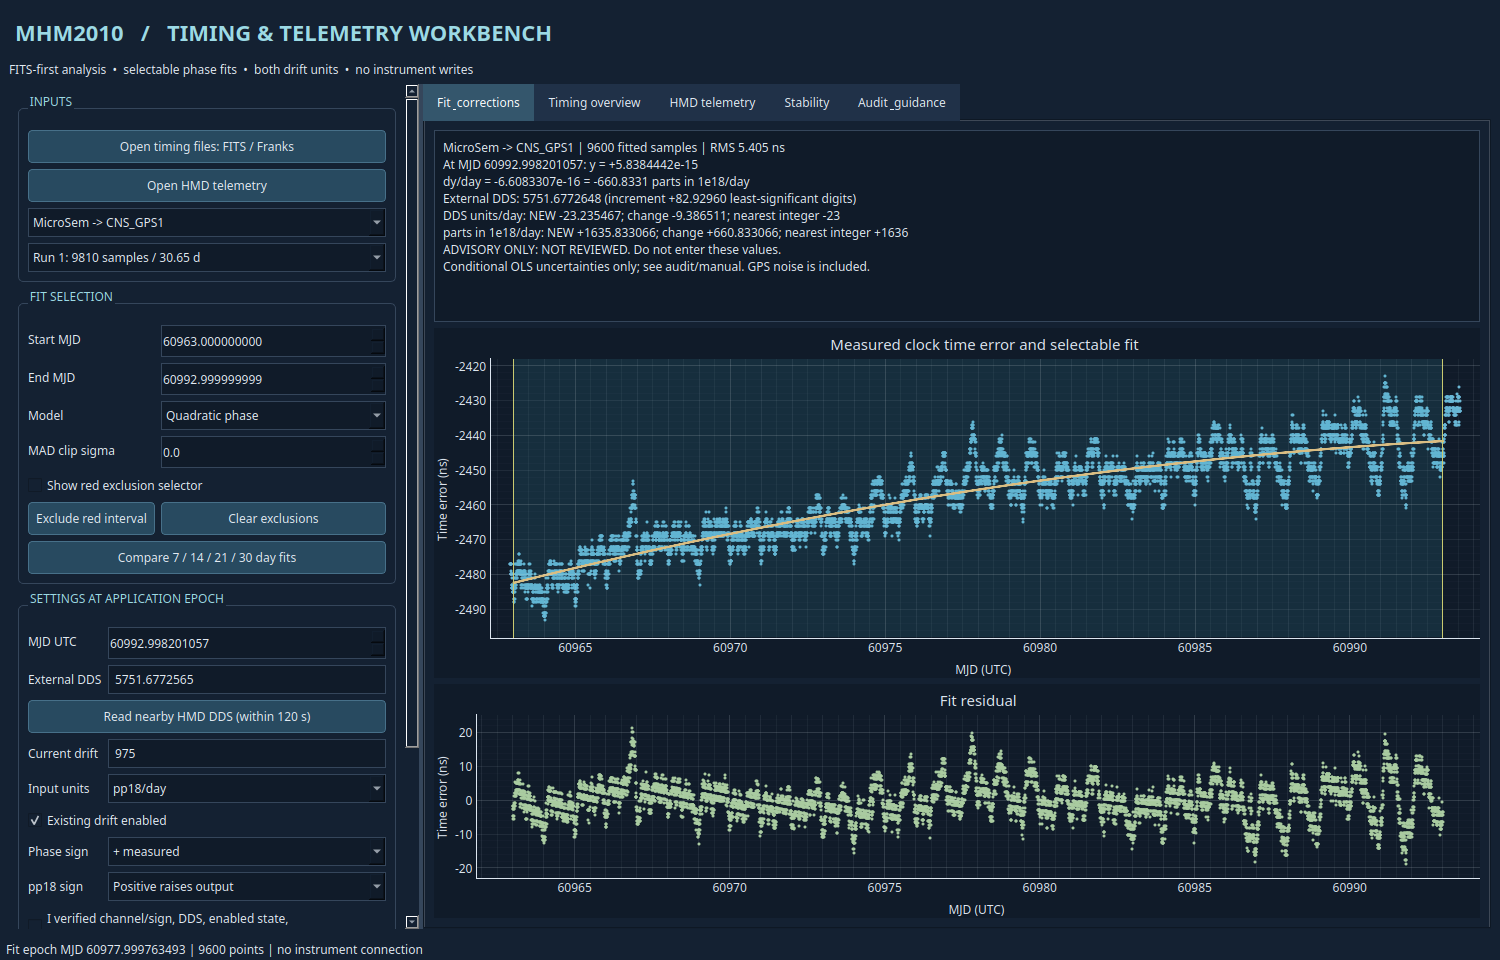
\includegraphics[width=\linewidth]{../validation/gui_fit.png}
\end{center}
\smallskip
\textbf{Fit and corrections tab.} The blue region selects the fitting interval.
The phase and residual plots share their horizontal view. Numeric MJD limits
provide precise selection without requiring a mouse.

The red region is an independent exclusion selector. Add its interval to the
exclusion list or clear the list. Excluded observations remain in the input
and export, with an explicit used-in-fit mask. Optional iterative MAD residual
clipping is disabled by default. It can reject outliers, but it changes noise
statistics and must not conceal physical events.

A linear phase model estimates frequency only; the drift field is not
estimated and should not be changed on that basis. A quadratic phase model
estimates frequency and frequency drift. Internal scaling improves numerical
conditioning without changing the physical units of the returned coefficients.

The 7/14/21/30-day comparison button reports trailing-window fits in the audit
tab. These are unclipped quadratic diagnostic fits, with actual span and
sample count shown. They are not confidence intervals.

\subsection{State and stale-result handling}
Changing the fit interval/model invalidates old stability results. Settings
can be saved without source-directory paths, then restored after selecting the
original files. Restoring settings clears operator acknowledgments. Export
creates a new folder; it never silently replaces an earlier result directory.

\warning{The plots are interactive analysis of selected files, not streaming
acquisition. Large file reads run outside the GUI thread; fitting, overview
construction and export may briefly occupy the GUI thread for very large
datasets. There is no serial or network maser interface in this release.}
\clearpage

\section{Correction interpretation and manual review}
\subsection{One epoch, two absolute settings}
The phase fit is centered on an internal reference epoch. Frequency error is
evaluated at the separate intended application epoch. The old DDS must be the
setting at that application epoch, not the setting at the start of the data
or at the centered fit epoch.

The new external DDS is an \textbf{absolute setting}, not a number to add
again. Its displayed increment is also reported in least-significant DDS
digits. The new drift is the existing enabled drift plus a residual correction,
with the sign and units handled explicitly. An existing disabled drift
contributes zero regardless of a stale numeric value in its field.

The pp18/day input field and DDS-units/day input field are alternative
representations of the same ramp. The program reports both new values and
both increments. Do not apply both increments sequentially.

\subsection{Sign and precision}
For the adopted timing definition, measured arrival(B) minus arrival(A)
equals clock(A) minus clock(B). A direct MicroSem-to-GPS pair therefore uses
the positive sign; a reverse pair uses the negative sign. This channel
interpretation must be checked against the installed measurement wiring and
logging convention.

Positive physical DDS units/day means the DDS number increases with time,
which lowers output frequency \manual. The installed pp18 sign is separately
selectable: positive raises output frequency, or positive raises DDS. The
default is an explicit assumption, not a claim that Rev. J documents that sign.

The external DDS is rounded to seven decimal places. Both drift values are
also shown without integer rounding and with nearest-integer alternatives.
The integer alternatives are illustrative: verify what entry precision the
installed masermon accepts. pp18 integer increments and DDS integer increments
do not have the same effective frequency-drift resolution.

\subsection{Before entering any candidate}
\begin{itemize}
\item \textbf{Reference}: confirm the GPS channel is healthy, not stepped or being steered unexpectedly.
\item \textbf{Instrument}: confirm external synthesizer selection, current DDS, drift enable state and units.
\item \textbf{Sign}: verify the instrument's installed pp18 convention; do not test it by an uncontrolled adjustment.
\item \textbf{Time}: use a current, defensible application epoch and known setting at that epoch.
\item \textbf{Fit}: inspect residuals, HMD changes, outages and window sensitivity.
\item \textbf{Record}: preserve old settings, intended values, operator review and subsequent comparison data.
\end{itemize}

No checkbox turns this software into a certified controller. Values remain
advisory even after the operator review fields are acknowledged.
\clearpage

\section{Stability analysis and Stable32}
OADEV, MDEV, TDEV and OHDEV use phase samples in seconds and the NIST SP 1065
definitions \nist. The calculation supports raw phase, mean removal, linear
phase removal and quadratic phase removal. Results are labeled with the chosen
detrending; raw stability must not be confused with fitted-residual stability.

The code validates both adjacent intervals and cumulative deviation from a
uniform grid. It never fills gaps or interpolates samples. The mean actual
interval establishes the nominal sampling period after validating the record.
The default relative tolerance is 1\%; the interface allows up to 5\%.
This is an explicit approximate-uniformity tolerance, not proof that jitter
has no effect at the shortest averaging times.

For the supplied month, a 2\% tolerance admits an approximately 3 s maximum
grid deviation on a 270 s cadence. The default 1\% rejects the full record.
An internal exclusion creates a missing interval and is not compressed away
to make a false uniform series.

At least ten contributing terms are required for each plotted estimate.
Overlapping terms are correlated; their count is not an equivalent number of
independent degrees of freedom. No confidence bands or maser-only noise
separation are claimed \nist.

\begin{center}
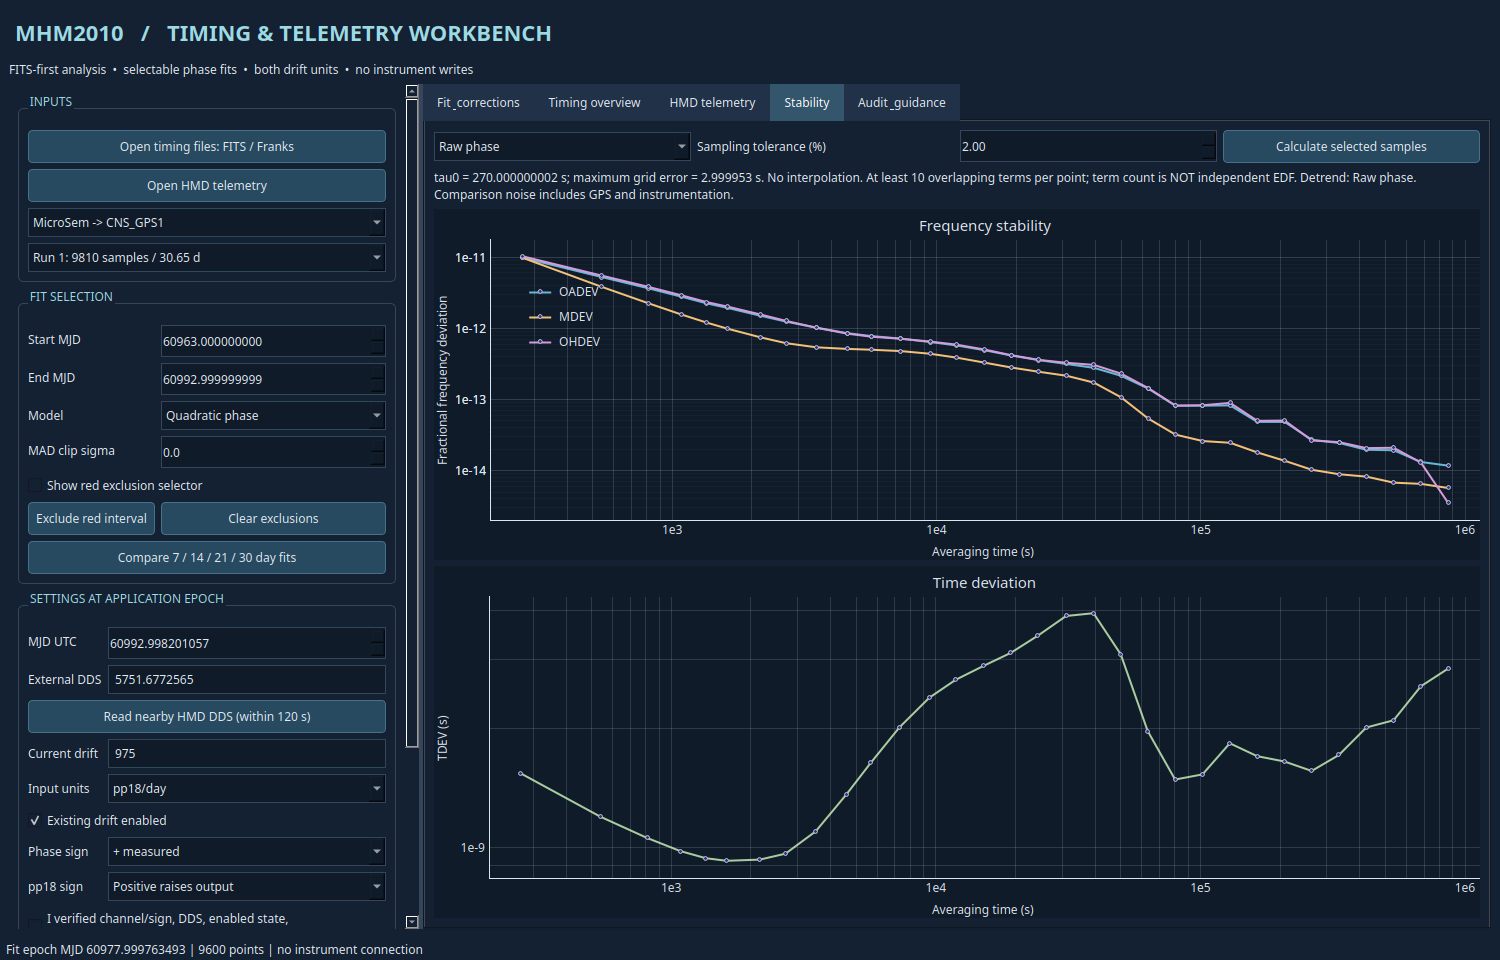
\includegraphics[width=.94\linewidth]{../validation/gui_stability.png}
\end{center}

\subsection{Stable32 files}
\texttt{raw.PHD} holds phase seconds and \texttt{raw.FRD} holds fractional
frequency derived from successive phase samples. The frequency record has one
fewer point. Fit-residual versions are written separately. The headers contain
type, point count and tau; companion CSV/JSON files retain original timestamps,
units, tolerance checks and export decisions \stablemanual.

Stable32 treats embedded zeros as gaps. Actual zeros are exported as
\texttt{1e-99}, following the manual's recommendation; replacements are counted
in the sidecar \stablemanual. Do not use its gap-fill controls to disguise a
nonuniform or incomplete input record.
\clearpage

\section{Output package and reproducibility}
\begin{longtable}{@{}p{.35\linewidth}p{.60\linewidth}@{}}
\toprule
Output & Meaning\\
\midrule
\texttt{analysis.vszh5} & Native HDF5 document, typed datasets and Veusz plotting script.\\
\texttt{analysis.json} & Fit, coefficients, conditional covariance, settings, both drift units, provenance and warnings.\\
\texttt{phase\_and\_fit.csv} & All input timing samples, model, residual, selection and fit masks.\\
\texttt{telemetry\_overlap.csv} & HMD rows overlapping the selected timing interval, if present.\\
\texttt{stability.csv} & Estimator, tau, deviation and overlapping-term count.\\
\texttt{raw.PHD / raw.FRD} & Optional uniform-record Stable32 phase and fractional frequency.\\
\texttt{fit\_residual.*} & Separately identified residual stability inputs.\\
\texttt{review.md} & Human-readable advisory summary and reference table.\\
\bottomrule
\end{longtable}

The HDF5 document is written using the supplied writer without importing
Veusz. All measured raw pair datasets and descriptive labels are included when
the full collection is exported. Overview medians are separate datasets.
The example's externally rendered PDF is a preview, not a dependency of the
application.

Exports first build in a temporary adjacent folder and rename only after
success. An existing destination is rejected. This protects earlier results
on ordinary local filesystems; no distributed-filesystem transactional
guarantee is claimed.

\subsection{Batch operation}
\begin{lstlisting}
python analyze_maser.py --fits-directory <FITS_DIRECTORY>
  --hmd <HMD_FILE> --start 2025-10-15 --end 2025-11-14
  --derive-dds --drift 975 --sampling-tolerance .02
  --stable32 --output <NEW_OUTPUT_DIRECTORY>
\end{lstlisting}
Join the lines for the shell. The end time is exclusive. Without DDS and drift
inputs, the batch path exports measurement results without a correction
candidate. \texttt{--derive-dds} only copies an HMD setting within 120 s of the
historical application epoch; it does not retrieve present-day state.

\subsection{Writer revision}
The attached writer was version 0.0.21. A targeted test demonstrated that
\texttt{dataset\_date()} accepted multidimensional input, creating invalid
date shape or silently flattening it in resizable mode. Version 0.0.22 adds
one-dimensional validation before creating the dataset group. Valid callers
retain the same API. This is a scoped defect correction, not an exhaustive
review of every writer feature.
\clearpage

\section{Historical validation results}
The uploaded archive contains 109 FITS.GZ files and 40 measured channel pairs,
9,810 records per pair. The example selects October 15 through November 13,
2025, producing 9,600 direct MicroSem-to-CNS\_GPS1 samples. The HMD record covers
April 9, 2025, through March 25, 2026. The previously supplied July 2026 timing
files do not overlap that HMD record.

At the last selected sample, November 13, 2025, 23:57:24.571 UTC, the quadratic
fit gives frequency error \(+5.83844\times10^{-15}\), residual drift
\(-660.833\) parts in \(10^{18}\)/day and phase-residual RMS 5.405 ns.
These are computed results from the supplied files, not external instrument
specifications.

\warning{The example assumes enabled drift \(+975\) pp18/day and a positive
pp18 sign that raises output frequency. The older screenshot supplies that
example number, but does not establish its value in November. The following
candidates are historical and unapproved.}

\begin{tabular}{@{}p{.49\linewidth}r@{}}
\toprule
Quantity & Historical example\\
\midrule
HMD DDS near the last timing sample & 5751.6772565\\
Calculated DDS increment, last digits & +82.929597\\
New rounded DDS & 5751.6772648\\
New drift, pp18/day & +1635.833066\\
Equivalent new drift, DDS units/day & -23.235467\\
Nearest integer pp18/day alternative & +1636\\
Nearest integer DDS units/day alternative & -23\\
\bottomrule
\end{tabular}

\subsection{The dominant warning: fit-window sensitivity}
\begin{tabular}{@{}rrrr@{}}
\toprule
Window, d & Frequency error at common end & Drift, pp18/day & RMS, ns\\
\midrule
30 & \(+5.83844\times10^{-15}\) & -660.833 & 5.405\\
21 & \(+3.80025\times10^{-15}\) & -883.575 & 5.810\\
14 & \(+1.39421\times10^{-14}\) & +407.199 & 5.922\\
7  & \(-4.32655\times10^{-15}\) & -5454.180 & 6.970\\
\bottomrule
\end{tabular}

The drift changes sign with the fitting interval. Conditional OLS errors are
much smaller than this variation and must not be interpreted as a complete
uncertainty budget. A longer/reference-checked operating-state review is
needed before any live adjustment.

For the 30-day window, CNS2018 and CNS\_GPS2 comparisons give \(-688.966\)
and \(-652.571\) pp18/day. Similar values are useful but do not demonstrate
independent references or isolate maser aging.
\clearpage

\section{Cross-checks, testing and limitations}
\subsection{Franks/Veusz comparison}
The supplied Veusz example was read as HDF5 data, without executing its
embedded plotting script. Across 735 matching UTC-hour bins in the full
archive span, the new derived MSM--GPS comparison differs by 1.284 ns RMS
from the historical reduced values. MicroSem and CNS\_GPS1 differ by
0.852 ns and 1.004 ns RMS. Median differences are approximately zero.
The maximum absolute differences are 4, 2 and 4 ns respectively.

These small differences are consistent with nonidentical reduction windows
and rounding, but that explanation is not a proof of identical processing.
The direct raw pair remains the primary correction input. Invalid negative
MJD legacy records and all-missing channels in the exemplar were not copied.

\subsection{Automated and rendering checks}
The delivered suite has 36 passing tests on Python 3.12. Tests cover analytic
phase coefficients, DDS direction, quantization, both drift representations,
disabled drift, reversal, duplicates, gap/grid rejection, clipping, FITS
metadata/padding, Franks sentinels, GUI controls/settings, writer behavior and
export protection.

OADEV, MDEV, TDEV and OHDEV were compared with AllanTools for seeded synthetic
phase data, including contributing-term counts. The 29-page historical
\texttt{.vszh5} was opened and rendered with a separate Veusz installation.
Its PDF has page bookmarks. GUI captures document the offscreen Qt tests.

\subsection{Not validated}
\begin{itemize}
\item \textbf{Windows/bracca}: actual desktop operation and local staging were not performed.
\item \textbf{Stable32 executable}: output structure was checked, but proprietary-application import remains a site test.
\item \textbf{Installed masermon}: sign, range, precision, update cadence, persistence and firmware/version behavior remain site checks.
\item \textbf{Physical system}: no live adjustment, calibration or post-adjustment monitoring was conducted.
\item \textbf{Uncertainty}: no colored-noise confidence intervals, reference-error removal or independent maser-aging measurement is claimed.
\end{itemize}

\subsection{Repository provenance}
The RF\_Equipment\_Comms stability-tool code
\href{https://github.com/Braveheart53/RF_Equipment_Comms/tree/main/sa_stability_tool}{[5]}
and FitsAutoPlot sources \href{https://github.com/Braveheart53/FitsAutoPlot}{[6]}
were read for header, GUI and analysis conventions. The science modules in this package
are new implementations using the cited definitions, not a wholesale copy of
the signal-analyzer tool. Repository checkouts were read-only with respect
to their remotes; no push was performed.

Reviewed commits:
\begin{itemize}
\item RF\_Equipment\_Comms: \texttt{9305e94e9ad85dbdb94a3765cf0989449dc3f345}.
\item FitsAutoPlot: \texttt{36add38d973bc07e920ff70680a139241c421f7c}.
\end{itemize}
The product-page pointer is
\href{https://www.microchip.com/en-us/product/mhm-2010}{Microchip MHM-2010 [7]}.
\clearpage

\section{Appendix A: Implemented equations}
\subsection{Time, phase and polynomial fit}
Let \(t\) be elapsed SI seconds, obtained by converting UTC timestamps through
TAI, and \(d\) elapsed days from fit epoch \(t_0\). The MJD plotting conversion
is only a civil-date coordinate; it is not used for elapsed-time derivatives.
\begin{align}
t_i-t_0&=\operatorname{TAI}(\operatorname{UTC}_i)-
          \operatorname{TAI}(\operatorname{UTC}_0),&
d_i&=(t_i-t_0)/86400, \tag{A1}\\
v_i&=86400(\mathrm{MJD}_i-54832),&
h_i&=\lfloor24\,\mathrm{MJD}_i\rfloor. \tag{A2}
\end{align}
Here \(v_i\) is the Veusz seconds coordinate relative to 2009-01-01 and \(h_i\)
indexes a UTC-hour reduction bucket. Within each nonempty bucket, time and
phase are reduced by their medians:
\begin{equation}
(\widetilde{\mathrm{MJD}}_h,\widetilde{x}_h)
=\left(\operatorname{median}_{i:h_i=h}\mathrm{MJD}_i,\,
       \operatorname{median}_{i:h_i=h}x_i\right). \tag{A3}
\end{equation}

With phase coefficients in nanoseconds and \(d\) in days:
\begin{align}
\widehat{x}(d)&=10^{-9}(c_0+c_1d+c_2d^2)\ \mathrm{s}, \tag{A4}\\
y(d)&=\frac{10^{-9}}{86400}(c_1+2c_2d),&
r\equiv\frac{dy}{dd}&=\frac{2c_2\,10^{-9}}{86400}\ \mathrm{day}^{-1}. \tag{A5}
\end{align}
For a linear fit, \(c_2\) is not estimated; the drift result is withheld, not
presented as evidence of zero physical drift.

Let \(s=\max_i|d_i|\), \(A_{ij}=(d_i/s)^j\), \(b_i=10^9x_i\), and let
\(T=\operatorname{diag}(1,s^{-1},s^{-2})\), truncated for a linear fit:
\begin{align}
\widehat{\boldsymbol\beta}&=\arg\min_{\boldsymbol\beta}
 \|A\boldsymbol\beta-\mathbf b\|_2^2,&
\mathbf c&=T\widehat{\boldsymbol\beta}, \tag{A6}\\
\widehat{\sigma}^2&=\frac{\sum_i e_i^2}{N-p},&
C_c&=T\left[\widehat{\sigma}^2(A^\mathsf{T}A)^{-1}\right]T^\mathsf{T},
 & e_i&=b_i-(A\widehat{\boldsymbol\beta})_i. \tag{A7}
\end{align}
Here \(p\) is coefficient count. The reported fit scatter and conditional
uncertainties are:
\begin{align}
\mathrm{RMS}_{\mathrm{ns}}&=\sqrt{\frac1N\sum_i e_i^2},&
\sigma_y&=\frac{10^{-9}}{86400}\sqrt{\mathbf g^\mathsf{T}C_c\mathbf g},
 &\mathbf g&=(0,1,2d)^\mathsf{T}, \tag{A8}\\
\sigma_r&=\frac{2\,10^{-9}}{86400}\sqrt{(C_c)_{22}}. \tag{A9}
\end{align}
They assume IID residuals conditional on the chosen fit; they do not represent
a full timing-standard uncertainty.
\clearpage

\subsection{Clipping, continuity and channel convention}
Optional clipping uses median-centered residuals and a robust scale:
\begin{equation}
M=\operatorname{median}(e),\quad
S=1.4826\,\operatorname{median}|e-M|,\quad
\text{retain }i\ \text{if}\ |e_i-M|\le kS. \tag{A10}
\end{equation}
There are at most eight clipping passes, followed by a final refit. \(k=0\)
disables clipping. A fitting run is split at gaps exceeding five median
timestamp intervals:
\begin{equation}
\Delta\mathrm{MJD}_i>5\operatorname{median}(\Delta\mathrm{MJD}). \tag{A11}
\end{equation}
These are software heuristics, not manufacturer operating limits.

For ideal pulse arrival times and clock time errors relative to the same
reference:
\begin{equation}
\Delta t_{A\rightarrow B}=t_{\mathrm{arrival},B}-t_{\mathrm{arrival},A}
=x_A-x_B,\qquad x_{\mathrm{maser-ref}}=\epsilon\,\Delta t,\quad
\epsilon\in\{-1,+1\}. \tag{A12}
\end{equation}
Fixed cable offsets affect the constant phase term; changing delays can affect
slope and drift and are not removed automatically.

\subsection{DDS correction and both drift units}
The manufacturer relationship is \manual:
\begin{equation}
f_o=\frac{f_m}{D},\qquad D=284.08+aN,\qquad a=2\times10^{-7}. \tag{A13}
\end{equation}
For old DDS \(N\), measured residual fractional frequency \(y\), and
least-significant DDS step \(q=10^{-7}\):
\begin{align}
k_N&=\frac{a}{D},&
\frac{\delta f_o}{f_o}&\simeq-k_N\delta N,&
g_{\mathrm{digit}}&=-k_Nq, \tag{A14}\\
\Delta N&=\frac{D}{a}y,&
N_{\mathrm{new}}&=\operatorname{round}_{q}(N+\Delta N),&
\Delta n&=\Delta N/q. \tag{A15}
\end{align}
Before rounding, the static relation exactly cancels the measured residual:
\begin{equation}
1+y_{\mathrm{new}}=(1+y)\frac{D}{D_{\mathrm{new}}},\qquad
D_{\mathrm{new}}=284.08+aN_{\mathrm{new}}. \tag{A16}
\end{equation}
The quantization residual is computed from (A16) with Decimal arithmetic.
The physical DDS rate \(v\), in last digits/day, transforms as:
\begin{equation}
v_{\mathrm{new}}=(1+y)v_{\mathrm{old}}+\frac{r}{k_Nq}. \tag{A17}
\end{equation}
Let \(P\) be the displayed pp18/day value and \(\eta=+1\) when positive \(P\)
raises output frequency, or \(-1\) when it raises DDS:
\begin{align}
v_{\mathrm{old}}&=-\frac{\eta P_{\mathrm{old}}10^{-18}}{k_Nq},&
P_{\mathrm{new}}&=-\eta\,v_{\mathrm{new}}\,k_{N,\mathrm{new}}q\,10^{18}, \tag{A18}\\
P_{\mathrm{new}}&\simeq P_{\mathrm{old}}-
       \frac{\eta r\,10^{18}}{1+y},&
k_{N,\mathrm{new}}&=a/D_{\mathrm{new}}. \tag{A19}
\end{align}
The code reports the rounded-DDS conversion in the both-units table.
An inactive old drift uses \(v_{\mathrm{old}}=0\). These equations describe
the local rate at the application epoch, not undocumented firmware scheduling.
\clearpage

\subsection{Rounding, uniformity and Stable32 conversion}
For nearest-integer drift alternatives:
\begin{align}
\delta r_v&=-(\operatorname{round}v_{\mathrm{new}}-v_{\mathrm{new}})
               k_{N,\mathrm{new}}q, \tag{A20}\\
\delta r_P&=\eta(\operatorname{round}P_{\mathrm{new}}-P_{\mathrm{new}})10^{-18}.
 \tag{A21}
\end{align}

For a record of \(N\) samples, interval tolerance \(\rho\), and time coordinates
from (A1), the validation is:
\begin{align}
\tau_0&=\frac{t_{N-1}-t_0}{N-1},&
\max_i\left|\frac{t_{i+1}-t_i}{\tau_0}-1\right|&\le\rho, \tag{A22}\\
\max_i|t_i-t_0-i\tau_0|&\le\rho\tau_0,&
0&<\rho\le0.05. \tag{A23}
\end{align}
At least eight finite matching samples are required. No missing interval is
compressed or interpolated. Stable32 fractional frequency and actual-zero
encoding are:
\begin{equation}
\overline y_i=\frac{x_{i+1}-x_i}{\tau_0},\qquad
z_{\mathrm{export}}=
\begin{cases}10^{-99},&z=0\ \text{(actual observation)},\\z,&z\ne0.\end{cases}
\tag{A24}
\end{equation}
The zero convention follows Stable32's documented gap handling \stablemanual.

\subsection{Stability estimators}
Let \(\tau=m\tau_0\), with integer \(m\ge1\), and \(x_i\) phase seconds.
All sums are over valid overlapping terms of a validated complete record.
The implementations follow NIST SP 1065 \nist:
\begin{align}
\sigma_y^2(\tau)&=
\frac{\sum_{i=0}^{N-2m-1}(x_{i+2m}-2x_{i+m}+x_i)^2}
     {2\tau^2(N-2m)}, \tag{A25}\\
\operatorname{mod}\sigma_y^2(\tau)&=
\frac{\displaystyle\sum_{j=0}^{N-3m}
 \left[\sum_{i=j}^{j+m-1}(x_{i+2m}-2x_{i+m}+x_i)\right]^2}
 {2m^2\tau^2(N-3m+1)}, \tag{A26}\\
\sigma_x(\tau)&=\frac{\tau}{\sqrt3}\operatorname{mod}\sigma_y(\tau), \tag{A27}\\
\sigma_H^2(\tau)&=
\frac{\displaystyle\sum_{i=0}^{N-3m-1}
(x_{i+3m}-3x_{i+2m}+3x_{i+m}-x_i)^2}
{6\tau^2(N-3m)}. \tag{A28}
\end{align}
The displayed OADEV, MDEV and OHDEV are square roots of the respective
variances. TDEV is (A27). Averaging factors are log-spaced integers, with
duplicates removed and at least ten contributing terms per reported point.
Optional detrending subtracts an OLS polynomial of order 0, 1 or 2 before
applying these equations; raw mode removes only a constant for numerical
convenience.
\clearpage

\section{What is new in release 0.2.2}
\begin{itemize}
\item \textbf{View $\rightarrow$ Time display (axes, dates, ranges)}: MJD (UTC), calendar date-time
local, or calendar date-time UTC, both ISO 8601 (e.g.\ \texttt{2026-11-05T15:47:13-05:00}). One choice
drives every time axis, every date field, the run list and the result text (next section).
\item \textbf{Fit windows}: ``Fit window'' presets and a Fit menu with the last 7, 14, 30 and 90 days
or all data, each offered only when the loaded data span it; comparison now includes 90 days.
\item \textbf{Veusz output named}: File $\rightarrow$ Export analysis folder (Veusz .vszh5, CSV, JSON,
Stable32) and Export T4 data (Veusz .vszh5, CSV, JSON); afterwards a dialog gives the
\texttt{.vszh5} path with Open in Veusz and Open folder (section ``Where the Veusz files are'').
\item MJD tick labels keep the decimals the spacing needs (61349.71, not 61349.7 twice); plot
titles are readable in the Light theme.
\end{itemize}

\section{Time display: MJD or ISO 8601 calendar time}
\subsection{Use}
Choose \textbf{View $\rightarrow$ Time display (axes, dates, ranges)}:
\begin{center}
\small
\begin{tabular}{@{}lll@{}}
\toprule
Menu entry & Example & Shortcut\\
\midrule
MJD (UTC) & \texttt{61349.86612} & Ctrl+Shift+M\\
Calendar date-time, local (ISO 8601) & \texttt{2026-11-05T15:47:13-05:00} & Ctrl+Shift+L\\
Calendar date-time, UTC (ISO 8601) & \texttt{2026-11-05T20:47:13+00:00} & Ctrl+Shift+U\\
\bottomrule
\end{tabular}
\end{center}

\includegraphics[width=.75\linewidth]{../validation/gui_view_time_display_menu.png}

The choice applies at once to: the fit, residual, HMD, overview, reference-figure, T4 telemetry and
T4 monitoring-file axes; the Start, End and application-epoch fields (they show and accept the chosen
form); the run list; the result text and status bar (calendar times keep the MJD in brackets for the
audit trail); and audit messages. It is remembered in \texttt{workbench\_view.ini} beside the program and
saved with the analysis settings. The data, fits and exported numbers are always MJD (UTC); only the
display changes. The \texttt{.vszh5} always contains every time page against both MJD and local ISO time.

\textbf{Typing a time.} In calendar modes a field accepts \texttt{2026-11-05T15:47:13-05:00}, the one-digit
offset \texttt{-5:00}, \texttt{Z}, a date alone, a time without offset (read as local in local mode, UTC in
UTC mode) or a plain MJD. Up/down steps one hour (one day in MJD mode). The batch script's
\texttt{--start}/\texttt{--end} accept the same forms (no offset = UTC).

\subsection{Conversion and ticks}
\[
t^{\mathrm{Unix}}=(\mathrm{MJD}-40587)\times86400\ \mathrm{s},\qquad
t^{\mathrm{local}}=t^{\mathrm{Unix}}+\Delta_{\mathrm{local}}(t^{\mathrm{Unix}}),
\]
with $\Delta_{\mathrm{local}}$ the computer's UTC offset at that instant ($-4$~h in summer, $-5$~h in
winter at Green Bank), so a July time shows \texttt{-04:00} and a November time \texttt{-05:00}. Ticks
fall on round calendar times (pyqtgraph's date logic, daylight-saving aware) and are labelled with
the full ISO time on two lines (date, then \texttt{Thh:mm:ss$\pm$hh:mm}); ticks closer than one label
width are dropped so labels never overlap. The axis title gives the offsets in the range, e.g.\
``Local date-time, ISO 8601 (UTC$-$05:00 then $-$04:00)''. ``Julian'' in common speech often means
this calendar view; strictly, MJD is the Julian-day count (JD$-$2\,400\,000.5) and the calendar
dates are Gregorian.

\begin{center}
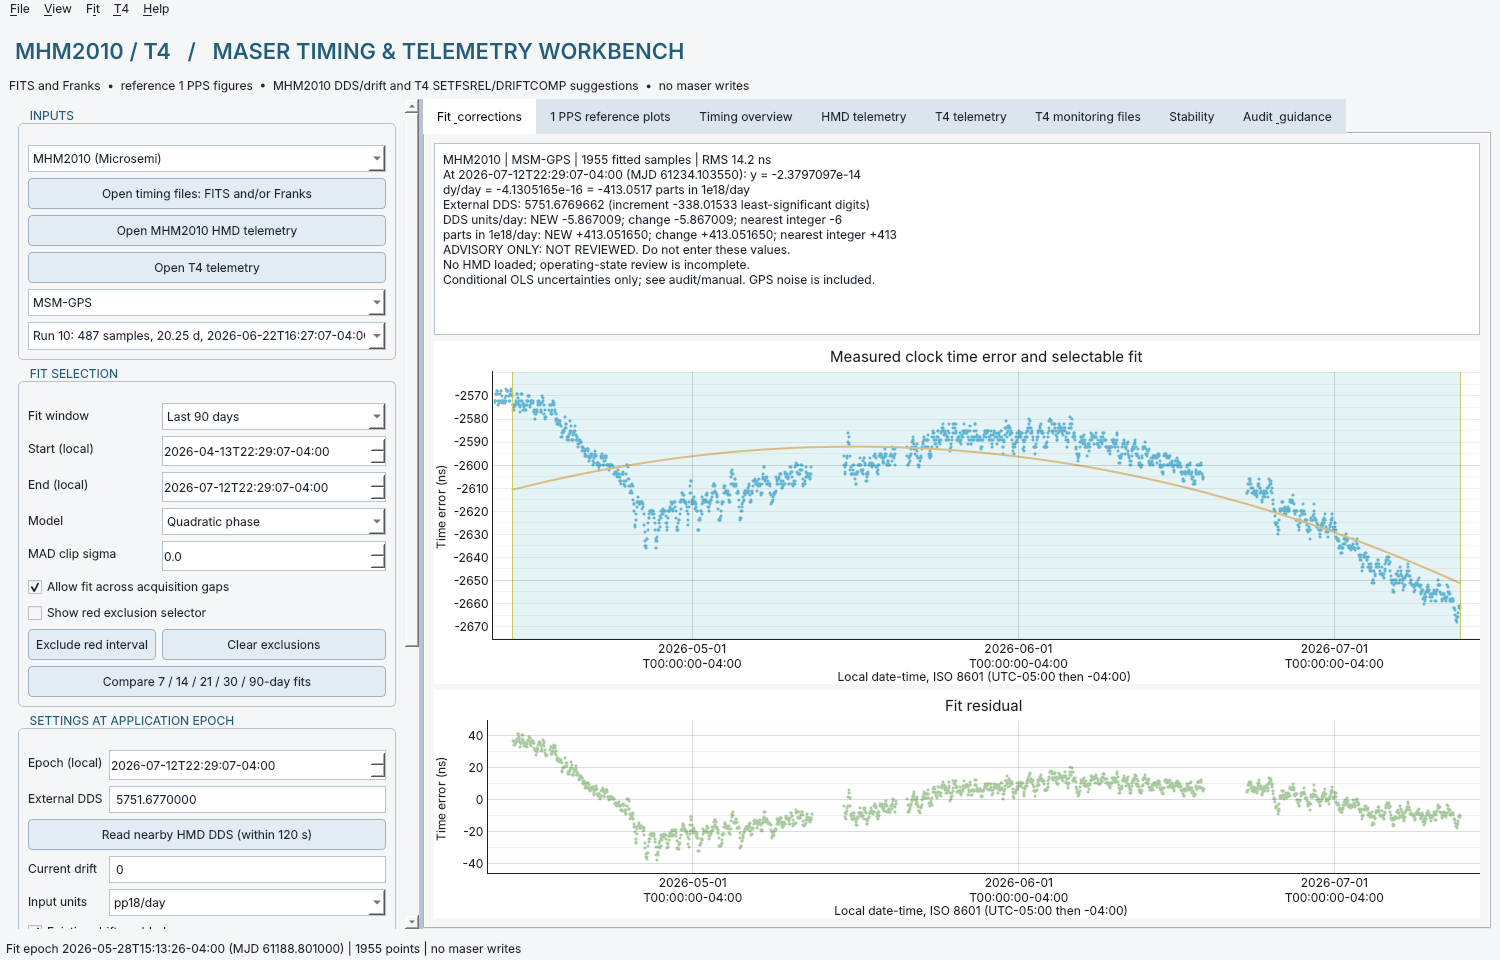
\includegraphics[width=.95\linewidth]{../validation/gui_time_display_local_90d_light.png}\\
{\small Local ISO 8601 display, last 90 days of the 2026 Franks MSM-GPS channel (Light theme).}
\end{center}

\section{Fit windows: last 30 and 90 days}
FIT SELECTION $\rightarrow$ \textbf{Fit window} (or the \textbf{Fit} menu) sets the blue interval to the
last 7, 14, 30 or 90 days ending at the last sample, or to all data, and moves the application epoch to
the last sample. A preset is enabled only when the loaded channel spans it (its tooltip gives the span
otherwise). If the window contains acquisition gaps, ``Allow fit across acquisition gaps'' is switched
on and logged; check the plot for phase steps. Dragging the blue interval returns to ``Custom''.
\textbf{Compare 7/14/21/30/90-day fits} (or Fit $\rightarrow$ Compare window lengths) fits each trailing
window ending at the selected end, skipping windows longer than the data; results go to the audit tab.
In batch, \texttt{--last-days 30} or \texttt{90} does the same and stops if the data are shorter.

On the 2026 Franks MSM-GPS data (193 days), the 90-day quadratic window ending 2026-07-13 02:29 UTC
gives $y=-2.38\times10^{-14}$ and drift $-413$ parts in $10^{18}$/day with 14.2~ns RMS; the 30-day
window gives $y=-3.71\times10^{-14}$, $-686$ parts in $10^{18}$/day and 3.6~ns RMS. The difference is
the window sensitivity this comparison exists to expose; the 90-day window spans gaps and a visible
phase excursion in April.

\section{Where the Veusz files are}
The \texttt{.vszh5} files are written only by an export, always into a \emph{new} folder:
\begin{center}
\small
\begin{tabular}{@{}p{.36\linewidth}p{.58\linewidth}@{}}
\toprule
Action & Result\\
\midrule
File $\rightarrow$ Export analysis folder (Ctrl+E), or OUTPUT $\rightarrow$ ``Export analysis: Veusz
.vszh5 + CSV/JSON'' & \texttt{<parent>/<MHM2010|T4>\_analysis\_}\allowbreak\texttt{<YYYYMMDDTHHMMSS$\pm$hhmm>/}\allowbreak\texttt{analysis.vszh5}
(needs a valid fit)\\
File $\rightarrow$ Export T4 data (Ctrl+Shift+E), or the T4 tabs' export buttons &
\texttt{<parent>/T4\_telemetry\_export\_<time>/}\allowbreak\texttt{t4\_telemetry.vszh5}\\
\texttt{analyze\_maser.py \dots --output DIR} & \texttt{DIR/analysis.vszh5} (path printed as
\texttt{veusz\_file})\\
\texttt{t4\_native.py FILES --output DIR} & \texttt{DIR/t4\_telemetry.vszh5}\\
\bottomrule
\end{tabular}
\end{center}
After a GUI export a dialog shows the full path with \textbf{Open in Veusz} and \textbf{Open folder};
``Open last export in Veusz'' (OUTPUT box and File menu) reopens it. Veusz is looked for at the path set
with File $\rightarrow$ Set Veusz program, then on PATH, then in
\texttt{Program Files\textbackslash Veusz}; if not found, the program asks once. Veusz 3.6 or later opens
\texttt{.vszh5} directly.

\begin{center}
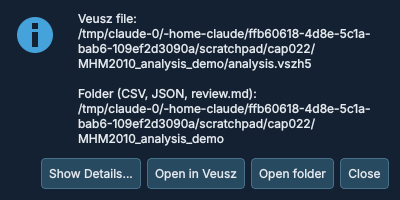
\includegraphics[width=.45\linewidth]{../validation/gui_export_dialog.png}
\end{center}

\section{What is new in release 0.2.1}
\begin{itemize}
\item \textbf{T4 monitoring files}: the LAN module's own logs from FTP \texttt{./Monitoring}
(e.g.\ \texttt{MonitHCB.dat}) are read by \texttt{t4\_native.py} 0.0.1, shown in a new tab
``T4 monitoring files'', exported (CSV, JSON, \texttt{.vszh5} against MJD and local time) and
added to analysis bundles. Format, time base and the clock-not-set rule are in the next sections.
\item \textbf{Local UDP port 14000} by default for live T4 polling (GUI and command line).
\item \textbf{Operator script} \texttt{tools/T4\_Reboot.py} 0.0.4 with loopback tests (it is not
part of the workbench, which still sends no settings).
\item \textbf{Corrections}: REBOOT restarts the M\&C software (\tfournet, Table~1, p.~8); manual
section and page citations checked page by page.
\end{itemize}

\section{What is new in release 0.2.0}
\begin{itemize}
\item \textbf{T4 iMaser 3000}: maser selector; SETFSREL and DRIFTCOMP suggestions from the
OEM relations \tfourman, \tfournet; a T4 telemetry tab that reads recorder files and text logs
and can poll the maser with read-only queries; a loopback emulator for tests and demonstrations.
\item \textbf{Reference 1 PPS figures}: the operator's two figures (deltas with statistics;
data and fit over residuals) in the GUI and as the first pages of every \texttt{analysis.vszh5}.
\item \textbf{FITS and Franks together}: one selection may hold both; they remain separate
series. Franks month-boundary repeats are resolved and reported; fits may bridge gaps.
\item \textbf{Time axes}: every time-series page exists against MJD (UTC) and against the
local date-time of the processing computer, with ISO~8601 tick labels [12]
(writer 0.0.24).
\item \textbf{GUI}: menu bar (File, View with Light/Dark theme, T4, Help).
\end{itemize}

\section{Reference 1 PPS figures}
\subsection{Definitions}
For the $N$ samples of a figure, $x_i=\mathrm{MJD}_i-\mathrm{MJD}_0$ (days, $\mathrm{MJD}_0$
the first sample shown) and $y_i$ is the 1 PPS time difference in ns. The deltas figure
uses every sample of the selected interval; the fit figure uses the samples actually
fitted (operator exclusions removed, drawn hollow and grey). The boxes report
\[
\bar y=\frac1N\sum_i y_i,\qquad
\mathrm{std}=\sqrt{\frac1N\sum_i (y_i-\bar y)^2}\quad(\text{population value, as \texttt{numpy.std}}).
\]

\subsection{Straight-line fit and its standard errors}
With $\bar x$, $S_{xx}=\sum(x_i-\bar x)^2$ and $S_{xy}=\sum(x_i-\bar x)(y_i-\bar y)$, the
least-squares line $y=a_1x+a_0$ minimizes $\sum r_i^2$, $r_i=y_i-a_1x_i-a_0$. Setting
$\partial/\partial a_0=\partial/\partial a_1=0$ gives the normal equations, whose solution is
\[
a_1=\frac{S_{xy}}{S_{xx}},\qquad a_0=\bar y-a_1\bar x .
\]
For independent residuals of variance $\sigma^2$, $\operatorname{Var}(a_1)=\sigma^2/S_{xx}$;
because $\operatorname{Cov}(\bar y,a_1)=0$,
$\operatorname{Var}(a_0)=\operatorname{Var}(\bar y)+\bar x^2\operatorname{Var}(a_1)
=\sigma^2\left(\frac1N+\frac{\bar x^2}{S_{xx}}\right)$. With
$s^2=\sum r_i^2/(N-2)$ in place of $\sigma^2$:
\[
s(a_1)=\frac{s}{\sqrt{S_{xx}}},\qquad s(a_0)=s\sqrt{\frac1N+\frac{\bar x^2}{S_{xx}}},\qquad
\text{rate}=r=\frac{a_1\,[\mathrm{ns/day}]\times10^{-9}}{86400\ \mathrm{s}} .
\]
These are conditional IID errors; colored noise and GPS systematics are not included \nist.
Check against the operator's figure: $N=741$, $s=3.49$~ns over 31 days gives
$S_{xx}\approx741\times31^2/12$, $s(a_1)\approx0.014$~ns/day and $s(a_0)\approx0.257$~ns, as printed.

\subsection{Synthesizer adjustment line}
\textbf{MHM2010.} Appendix A gives the fractional change per DDS unit,
$\partial y/\partial D=-2\times10^{-7}/(284.08+2\times10^{-7}D)$ \manual. One count is
$10^{-7}$ DDS units, so cancelling $y=\sigma r$ ($\sigma=\pm1$ the phase sign) requires
\[
\Delta n=\frac{-\sigma r}{-2\times10^{-14}/(284.08+2\times10^{-7}D)}
=\frac{\sigma r\,(284.08+2\times10^{-7}D)}{2\times10^{-14}} .
\]
For $r=-3.15\times10^{-14}$ this is $-447$ counts, the value in the operator's figure; the
full DDS calculation of Appendix A agrees to $10^{-9}$ relative (test suite).

\textbf{T4.} The line shows the SETFSREL entry and the synthesizer change of the next
section for the same straight-line rate.

\warning{The figure's adjustment uses the straight-line mean rate over the plotted span, as
the operator's figures do. The settings panel evaluates the selected model (linear or
quadratic) at the application epoch. With a quadratic fit the two can differ; enter only
the reviewed settings-panel values.}

\begin{center}
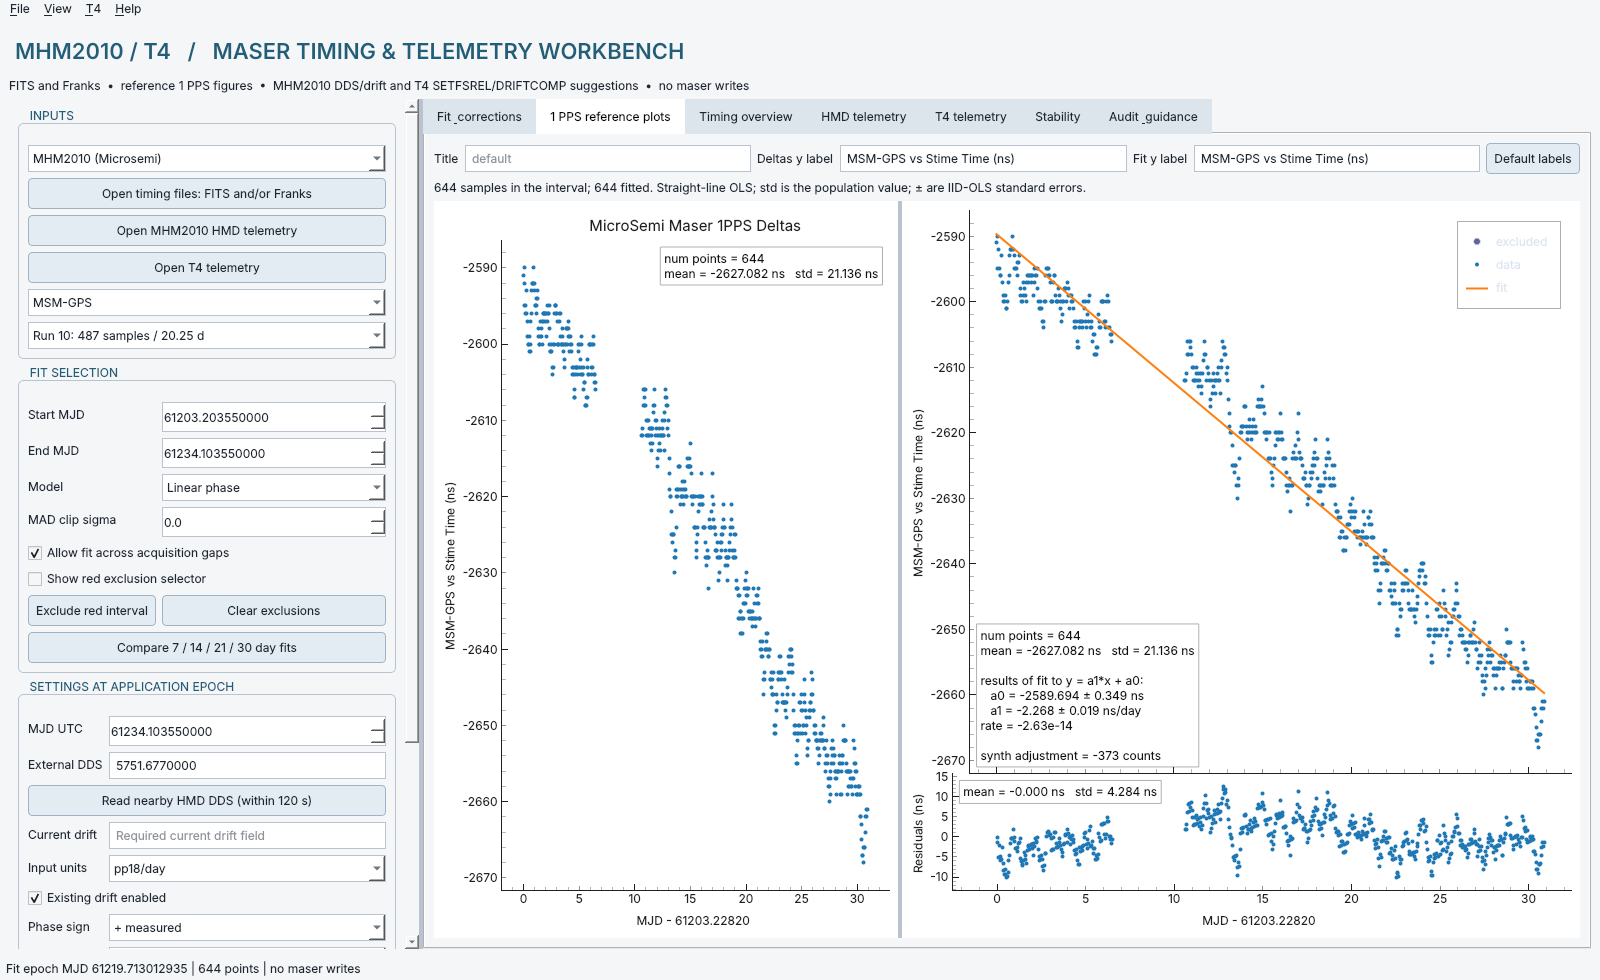
\includegraphics[width=\linewidth]{../validation/gui_reference_light.png}\\
{\small GUI tab ``1 PPS reference plots'' (Light theme) on the operator's Franks files,
June--July 2026, MSM-GPS.}
\end{center}

\section{FITS and Franks inputs together}
\begin{itemize}
\item FITS series are raw channel pairs keyed ``A -> B''; Franks series are hourly medians keyed
by column (e.g.\ \texttt{MSM-GPS}). Keys cannot collide; nothing is merged or interpolated.
\item \textbf{Month boundaries.} Consecutive \texttt{YYYY\_MM.t00new} files repeat the first hours
of the next month. Identical repeats are dropped. A disagreeing repeat (found in the supplied
files at MJD 61222.01917, Site1Hz 0 vs 1) keeps the row from the file named for that row's month,
and the conflict is listed in the audit tab.
\item \textbf{Gaps.} The 0.1.0 rule refused a fit across an acquisition gap. ``Allow fit across
acquisition gaps'' (default on for Franks data) fits through gaps and reports each one. The
supplied 2026 MSM-GPS series has nine gaps of 5 to 99 h; inspect the residuals for a phase step.
\end{itemize}

\section{T4 iMaser 3000}
\subsection{MONIT telemetry}
The reply to \texttt{MONIT;} is \texttt{\$} + 113 hexadecimal characters + CR LF (Type 1, Card
FPGA T4S-724) or CR (Type 2, IO card LAN T4S-711) \tfourman. The channels are 32 of 12 bits,
8 of 8 bits and the main-PLL lock bit:
\[
L_{\mathrm{hex}}=32\cdot3+8\cdot2+1=113,\qquad v_i=g_i\,c_i,\quad c_i=\texttt{int}(\text{field}_i,16)\ \text{(unsigned)}.
\]
Gains $g_i$ are Table 6 of \tfourman, identical to the operator's repository table \tfoursrc;
the $-15$~V rail has a negative gain. Channels 21, 37 and 39 are ``Not used''. Channel 40
(LOCK 100~MHz) is an 8-bit analog voltage; channel 41 is the lock bit (1 locked, 0 unlocked;
any other code is flagged). Decoding the manual's example reply gives 4.765~V for channel 40;
the operator's web-page screenshot shows 4.764~V.

\textbf{Inputs.} The recorder's \texttt{t4\_raw\_frames.csv} (re-decoded from the raw replies),
its \texttt{t4\_telemetry.csv} (raw codes re-scaled), or text logs with one
\texttt{<time> \$<frame>} per line. Times must be MJD or ISO~8601 with an offset.

\textbf{Live polling} (T4 tab) sends only \texttt{MONIT;}, \texttt{RDFS;}, \texttt{GETID;} and
\texttt{RDREG=\dots;} over UDP port 14000 \tfournet. Each attempt uses a fresh socket with bounded
retries; datagrams from other peers are ignored. Since 0.2.1 the local UDP port defaults to
14000 for a real T4: the vendor example and \texttt{T4\_Maser\_Comms.py} bind it (``seems one
must bind the port to local port as well'' \tfoursrc), so the T4 probably answers to port 14000
rather than to the sender's port; the manual does not say. The emulator uses an ephemeral port. Raw replies are written before decoding, into a
folder stamped once at creation (\texttt{T4\_telemetry\_YYYYMMDDTHHMMSS±hhmm}). The preview buffer
is bounded and can be flushed or offloaded to a pickle. A non-loopback address requires the
approval box. ``Use loopback emulator'' serves the manual's example reply.

\subsection{Frequency setting: SETFSREL}
The PLL forces the last IF to equal the synthesizer frequency, $\nu_{\mathrm{synth}}=F_{\mathrm{out}}-284\,\nu_{\mathrm{ocxo}}$,
and the output is the 5~MHz OCXO, $\nu_0=\nu_{\mathrm{ocxo}}=(F_{\mathrm{out}}-\nu_{\mathrm{synth}})/284$
(\tfourman, Eqs.~10--11). Differentiating at fixed $F_{\mathrm{out}}$:
\[
y_0=\frac{\Delta\nu_0}{\nu_0}=\frac{-\Delta\nu_{\mathrm{synth}}}{284\times5\ \mathrm{MHz}}
=\frac{-\Delta\nu_{\mathrm{synth}}}{1.42\times10^{9}\ \mathrm{Hz}}\qquad(\text{Eq.~12}).
\]
To cancel a measured offset $y$ the output must change by $\Delta y=-y$, so
$\Delta\nu_{\mathrm{synth}}=y\times1.42\times10^{9}$~Hz. The synthesizer resolution is
39 bits of 5~MHz (Sec.~9.4), $\delta=5\ \mathrm{MHz}/2^{39}=9.0949\times10^{-6}$~Hz
($6.405\times10^{-15}$ relative). The suggestion is quantized:
\[
n=\operatorname{round}\!\left(\frac{\Delta\nu_{\mathrm{synth}}}{\delta}\right),\qquad
\Delta y_{\mathrm{realized}}=-\frac{n\,\delta}{1.42\times10^{9}\ \mathrm{Hz}},\qquad
\texttt{SETFSREL}=\pm\Delta y_{\mathrm{realized}} .
\]
\tfournet\ defines SETFSREL as a relative step in s/s with a mandatory sign (range
$\pm29\times10^{-9}$), but not whether $+$ raises the output. The selector
``SETFSREL sign'' sets the convention, and the panel predicts the new \texttt{RDFS} value,
$\nu_{\mathrm{synth}}+n\delta$, which must lie within 405\,708--405\,795~Hz. \textbf{After entry, compare
RDFS with the prediction}; a move in the opposite direction means the convention is
reversed. RDFS values near 1.42~GHz (the web page's FREQ) are reduced by $1.42\times10^9$~Hz.

\subsection{Drift: DRIFTCOMP}
With linear drift, $y(t)=y_0+\dot y t$ and $x(t)=x_0+y_0t+\tfrac12\dot y t^2$ (\tfourman, Eqs.~22--23).
The quadratic phase fit $x=c_0+c_1d+c_2d^2$ (ns, days) gives
$y=(c_1+2c_2d)\times10^{-9}/86400$ and a drift per day
$\dot y_{\mathrm{day}}=2c_2\times10^{-9}/86400$. ``A positive sign will generate a positive slope
compensation'' \tfournet, so
\[
\texttt{DRIFTCOMP}_{\mathrm{new}}=\texttt{DRIFTCOMP}_{\mathrm{now}}-\sigma\,\dot y_{\mathrm{day}},
\qquad 10^{-17}<|\texttt{DRIFTCOMP}|<8\times10^{-13},
\]
followed by REBOOT, which ``Reboot[s] the M\&C software'' (\tfournet, Table~1, p.~8), and
\texttt{RDREG=DRIFTCOMP;} to verify. Neither command
removes the 1~PPS time offset (ADJ1PPS/SYNCPPS).

\begin{center}
\small
\begin{tabular}{@{}lr@{}}
\toprule
Demonstration (MSM-GPS used as a stand-in, \emph{not} T4 data) & Value\\
\midrule
Fit: last 30.9 d of 2026 Franks MSM-GPS, quadratic, gap bridged & 644 samples\\
$y$ at MJD 61234.10355 & $-3.7365\times10^{-14}$\\
$\Delta\nu_{\mathrm{synth}}$, steps & $-54.570~\mu$Hz, $-6$\\
Suggested entry (``+ raises output'') & \texttt{SETFSREL=+3.843E-14;}\\
RDFS before $\rightarrow$ predicted after & 405750.927598720 $\rightarrow$ 405750.927544150 Hz\\
Drift entry (current 0) & \texttt{DRIFTCOMP=+7.11e-16;}\\
\bottomrule
\end{tabular}
\end{center}

\warning{No FITS pair or Franks column is identified as the T4 yet. Designate the channel
in the GUI (``Selected channel is the T4 comparison'') or with \texttt{--maser T4 --channel}.
T4 settings stay blocked until the channel is designated.}

\section{T4 monitoring files (FTP ./Monitoring)}
\subsection{What the manual says}
\texttt{RECMONIT=<s>;} records the monitoring ``in a file stored on the local SD memory card'';
the file ``can be accessed by FTP under the directory ./Monitoring''; at 2~MB it ``is copied
with a tag of the date and time, and the current file is reset'' (\tfournet, Sec.~1.1.3, p.~12;
Sec.~6.5, p.~22). RECMONIT appears only in Sec.~1.1.3, not in the Table~1 command list. The web
page shows only whether recording is ON or OFF (Sec.~1.1.3, p.~12; Sec.~4, p.~20). Each record
is tagged with the module's date and time, set by NTP or \texttt{SETDATE}/\texttt{SETTIME}; without
synchronisation at power-up the clock is not kept (pp.~12, 22). Option telemetry such as the HCB
is recorded in these files although \texttt{MONIT} does not return it (p.~14). The FTP login is in
Sec.~6.1 (p.~21). The manual does not document file names, columns or the record layout.

\subsection{Format, as found in the GBO file}
\begin{center}
\small
\begin{tabular}{@{}p{.25\linewidth}p{.69\linewidth}@{}}
\toprule
Property & \texttt{MonitHCB.dat}, GBO T4, received 2026-11-05\\
\midrule
Layout & Tab-separated; CR~LF; header \texttt{TIME} then \texttt{Label [unit]} per column\\
Encoding & UTF-8; the degree sign arrived as U+FFFD (bytes EF BF BD) and is repaired to \textdegree\\
Time & \texttt{DD/MM/YY HH:MM:SS}, UTC, 1~s resolution\\
Records & 84: 10 before the time-server sync (3 stamped 2006-01-16, 7 stamped 2007-06-06), then 74
from 17:13:09 to 18:25:39 UTC\\
Interval & median 60~s, mean 59.59~s, range 59--62~s\\
Columns & Set, Internal and External temperature [\textdegree C]; Alarm Status (text)\\
\bottomrule
\end{tabular}
\end{center}
\textbf{Date order.} \texttt{16/01/06} cannot be MM/DD (no month 16), and YY/MM/DD would date the
newest records to 2005. The last record, 05/11/26 18:25:39, was 1.5~min before the file reached
this computer (13:27 EST = 18:27 UTC), consistent with UTC as the operator stated. DMY is the
default; the reader warns when another order would read every line that the chosen order cannot
(a wrong order can still read most lines: \texttt{05/11/26} is a valid MM/DD/YY).

\textbf{Time base.} With $t^{\mathrm{Unix}}$ the record time in seconds since 1970-01-01 UTC,
\[
\mathrm{MJD}=\frac{t^{\mathrm{Unix}}}{86400\ \mathrm{s}}+40587 ,
\]
so 2026-11-05 17:13:09 UTC is MJD $61349+\frac{62\,089}{86\,400}=61349.717465$. These are the
maser's own stamps (unlike MONIT rows, which carry this computer's receive time) and may be
compared with timing data directly.

\subsection{Clock not set}
A record is \emph{clock-valid} if $t_{\mathrm{min}}\le t\le t_{\mathrm{now}}+1$~d, with
$t_{\mathrm{min}}$ = 2020-01-01 UTC by default (``Clock valid from'' in the tab,
\texttt{--t4-earliest-valid} in batch). Other records are listed in the table and CSV (greyed,
\texttt{clock\_valid}=0, with their file and line) but never plotted or analysed. Runs of such
records are reported separately; a new run starts at a jump of more than 1~h or backwards. Interval
statistics use clock-valid records only: for successive stamps $t_k$,
$\Delta_k=t_{k+1}-t_k$, the median, mean, minimum and maximum of $\Delta_k$, the count of
$\Delta_k<0$, and the count of $\Delta_k>1.5\,\mathrm{median}(\Delta)$ (gaps).

\subsection{HCB columns}
HCB is the Active Heater-Cooler-Box option (climatic chamber) [13]; the SMC unit sets the
temperature of the liquid circulating in its tubes (\texttt{SETTEMPHCB}). The HTML page shows ``the
setting of the temperature'', ``the internal temperature sensor used for regulation'', ``the
external temperature sensor if used'' and ``the operation status normal or Alarm (the error code
of the error will be displayed)'' (\tfournet, Sec.~1.1.3, p.~16). In the GBO file, set point and
internal temperature are 21.5~\textdegree C throughout the clock-valid span (22~\textdegree C in the
2006 pre-sync records), the external temperature is a constant 80~\textdegree C, and the status is
``No error''. A constant 80~\textdegree C suggests that no external sensor is connected; this is an
inference, not confirmed. Status text is kept as written and plotted as a flag: 0 for ``No error'',
1 otherwise.

\subsection{Reading several files}
Files with the same header (the live file and its rolled, date-tagged copies) are merged in order of
their latest record, so a pre-sync 2006 stamp cannot put the newest file first. Identical records
(same time and values) are kept once; records with the same time but different values are kept and
reported. Files with different headers stay separate logs. Files are read in parallel threads; at
most 2~MB each \tfournet, they need no special memory handling, and ``Clear from RAM'' releases them.

\subsection{Outputs and use}
\begin{itemize}
\item \textbf{GUI}: open with File $\rightarrow$ Open T4 telemetry or monitoring files (Ctrl+T), the
T4 menu, or drag and drop; files are routed by content (a tab-separated header starting with
\texttt{TIME}). The tab shows one x-linked plot per column against $\mathrm{MJD}-\mathrm{MJD}_0$,
UTC or local date-time, the summary and notes, and every record.
\item \textbf{Export}: \texttt{t4\_<layout>\_records.csv} (every record, clock flag, source line;
UTF-8 with BOM), \texttt{t4\_telemetry.json}, and \texttt{t4\_telemetry.vszh5} with one panel per
column (each with its own range, padded by 10\,\% or $\pm0.5$ when constant), a status page and a
notes page, each against $\mathrm{MJD}-\mathrm{MJD}_0$ and against local ISO time.
\item \textbf{Batch}: \texttt{analyze\_maser.py --t4-telemetry MonitHCB.dat \dots} adds the pages to
\texttt{analysis.vszh5}; \texttt{python t4\_native.py MonitHCB.dat --output NEW\_DIR} exports only
the monitoring files.
\end{itemize}

\begin{center}
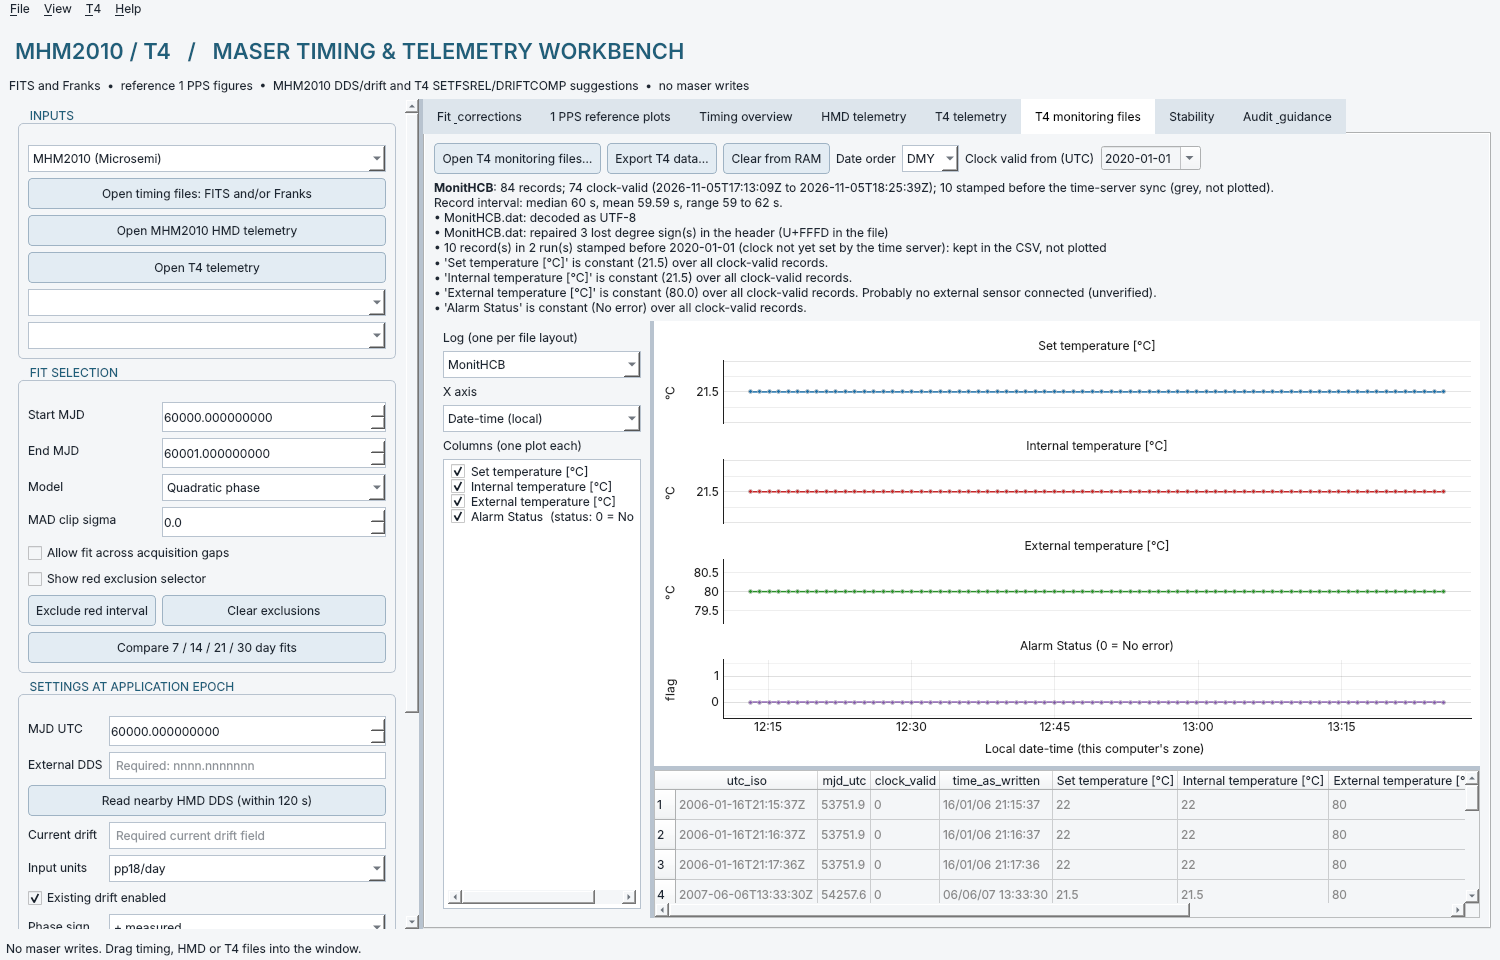
\includegraphics[width=.92\linewidth]{../validation/gui_t4_monitoring_light.png}\\
{\small Tab ``T4 monitoring files'' (Light theme, local date-time axis) on the GBO
\texttt{MonitHCB.dat}.}\\[6pt]
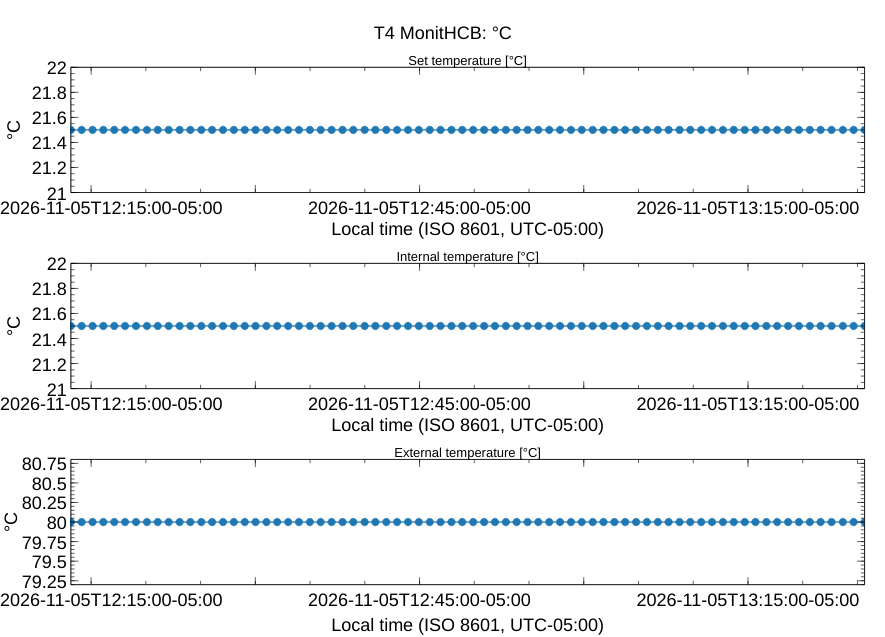
\includegraphics[width=.7\linewidth]{../validation/veusz_render_v0.2.1/t4_telemetry_p01_t4log0_monithcb_unit0_local.png}\\
{\small Veusz 3.6.2 render of the exported page against local ISO time (EST).}
\end{center}

\warning{The format is inferred from one HCB file. The main 40-channel monitoring file has not been
seen; the reader is header-driven and should read it if it has the same layout, but this is
untested. HCB alarm codes are not documented here.}

\section{Operator script: tools/T4\_Reboot.py}
The workbench sends no settings and no REBOOT. \texttt{tools/T4\_Reboot.py} 0.0.4 is a separate
operator script that reboots the M\&C software after checks; it is untested on a real T4.
\begin{enumerate}[leftmargin=6mm]
\item Read-only checks \texttt{GETID;}, \texttt{RDFS;}, \texttt{RDREG=DRIFTCOMP;} from local port
14000. Each answer must start with \texttt{\$} and the command; \texttt{!<command>} is a rejection
(\tfournet, Sec.~1.1.2, p.~11). Any failure stops the script before REBOOT.
\item The operator types \texttt{REBOOT}; the command is sent once. Table~1 lists no answer, so
silence is the expected result; \texttt{!REBOOT} stops the script.
\item After 30~s (the manual's wait after a front-panel reset, Sec.~6.7, p.~24; none is given for
REBOOT) the checks are repeated and compared. RDFS may change on its own when drift compensation
steps the synthesizer.
\end{enumerate}
Exit codes: 0 success or cancelled, 1 pre-check failed (nothing sent), 2 post-check failed,
3 REBOOT rejected or not sent. The original 0.0.1 script waited for a reply to REBOOT and therefore
ended with \texttt{TimeoutError} even when the reboot worked (reproduced on loopback). Sec.~1.1.3
(p.~13) describes REBOOT as ``Reset the LAN module'' and Sec.~6.7 (p.~24) says the equivalent
telnet reset ``will not affect the stability or the 1PPS generation''; confirm 1~PPS after a reboot.

\section{MJD and local ISO 8601 time axes}
Veusz stores dates as naive seconds from 2009-01-01; a local wall-clock axis is therefore
\[
V_i=t_i^{\mathrm{Unix}}-1\,230\,768\,000\ \mathrm{s}+\Delta_{\mathrm{local}}(t_i),\qquad
t^{\mathrm{Unix}}=(\mathrm{MJD}-40587)\times86400\ \mathrm{s},
\]
where $\Delta_{\mathrm{local}}$ is the processing computer's UTC offset, evaluated per sample
(daylight saving aware). The tick format is \verb|%VDY-%VDm-%VDdT%VDH:%VDM:%VDS| followed by
the offset, e.g.\ \texttt{2026-11-03T06:31:15-05:00}. Veusz formats are static, so when the data
cross a DST change the ticks omit the offset and the axis label lists each offset and when it
begins. Each time-series page is written twice (\texttt{\dots\_mjd}, \texttt{\dots\_local}); the
reference figures keep the operator's $\mathrm{MJD}-\mathrm{MJD}_0$ axis and gain
\texttt{pps\_deltas\_local} and \texttt{pps\_fit\_local}. Writer helpers: \texttt{mjd\_to\_epoch},
\texttt{local\_time\_axis}, \texttt{iso\_local\_strings}, \texttt{time\_pair\_pages}.

\begin{center}
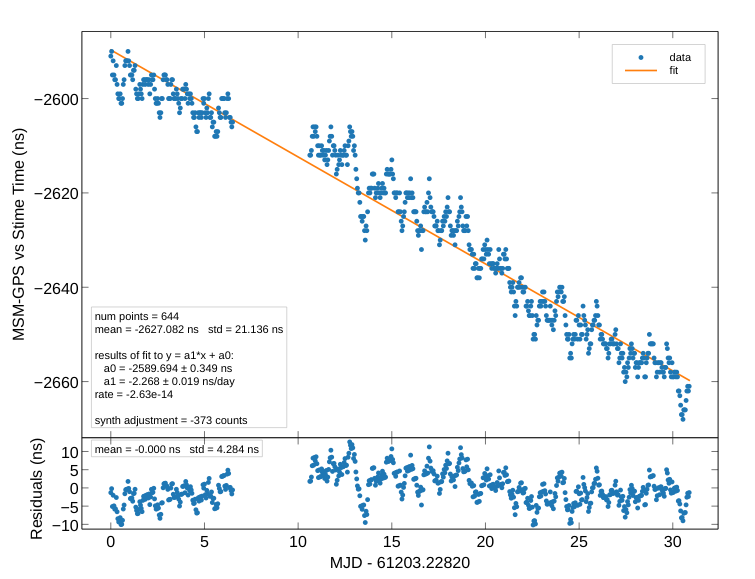
\includegraphics[width=.8\linewidth]{../validation/veusz_render_v0.2.0/analysis_p01_pps_fit.png}\\[4pt]
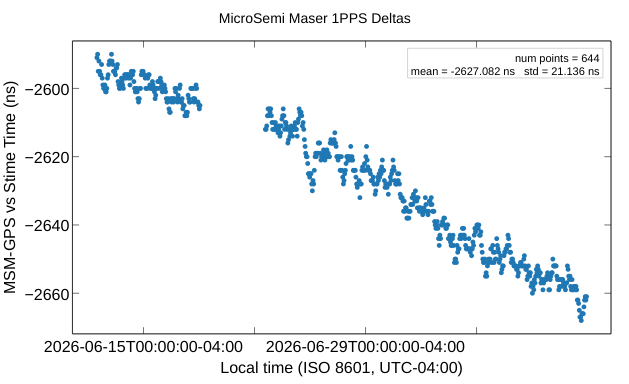
\includegraphics[width=.62\linewidth]{../validation/veusz_render_v0.2.0/analysis_p02_pps_deltas_local.png}\\
{\small Rendered by Veusz 3.6.2 from \texttt{analysis.vszh5}: fit page against
$\mathrm{MJD}-\mathrm{MJD}_0$, and the deltas twin against local ISO time (EDT in June).}
\end{center}

\section{Validation of release 0.2.2}
\begin{center}
\small
\begin{tabular}{@{}p{.42\linewidth}p{.5\linewidth}@{}}
\toprule
Check & Result\\
\midrule
Test suite (Python 3.12, PySide6 6.12.0, offscreen, TZ America/New\_York) & 112 passed: 103 from 0.2.1 + 9 time-display, fit-window and export tests\\
ISO 8601 round trip & \texttt{2026-11-05T15:47:13-5:00} $\rightarrow$ MJD 61349.866123 $\rightarrow$ \texttt{2026-11-05T15:47:13-05:00} / \texttt{20:47:13+00:00}; July shows \texttt{-04:00}\\
Every control follows the menu & axes, Start/End/epoch fields, run list, results, status bar, reference, T4 and monitoring tabs\\
Last 30 / 90 days, 2026 Franks MSM-GPS & 622 / 1955 samples; 90 d needs and enables gap bridging; disabled on the 12-day July file\\
Batch \texttt{--start} with \texttt{-4:00} offset & runs; \texttt{veusz\_file} printed; \texttt{--last-days 400} refused\\
\bottomrule
\end{tabular}
\end{center}
\textbf{Not validated:} Windows (time-zone rules come from the operating system there), launching
Veusz from the dialog (not installed in the test environment).

\section{Validation of release 0.2.1}
\begin{center}
\small
\begin{tabular}{@{}p{.42\linewidth}p{.5\linewidth}@{}}
\toprule
Check & Result\\
\midrule
Test suite (Python 3.12, PySide6 6.12.0, offscreen) & 103 passed: 79 from 0.2.0, 9 monitoring-file, 15 reboot-script (loopback)\\
GBO \texttt{MonitHCB.dat} & 84 records; 74 clock-valid, 17:13:09--18:25:39 UTC; 10 pre-sync in 2 runs; interval 59--62~s\\
Date order & DMY reads every line; MDY loses 3 lines and the reader warns\\
Franks 2026 regression with the file added & unchanged: $N=644$, $a_1=-2.268\pm0.019$ ns/day, $-373$ counts\\
Veusz 3.6.2 render of the monitoring export & 5 pages (per-column, status, notes; MJD and local)\\
\bottomrule
\end{tabular}
\end{center}
\textbf{Not validated:} the main 40-channel monitoring file, the reply port of the real T4, and the
reboot script on the real T4.

\section{Validation of release 0.2.0}
\begin{center}
\small
\begin{tabular}{@{}p{.42\linewidth}p{.5\linewidth}@{}}
\toprule
Check & Result\\
\midrule
Test suite (Python 3.12.15, PySide6 6.12.0) & 79 passed: 36 retained from 0.1.0, 29 T4, 10 reference/Franks/time/export, 4 GUI\\
Manual example MONIT replies (Type 1 and 2) & Decoded; channel 40 4.765 V vs 4.764 V on the web page\\
Franks 2026, MSM-GPS, last 30.9 d, linear & $N=644$, $a_1=-2.268\pm0.019$ ns/day, rate $-2.63\times10^{-14}$, $-373$ counts (DDS calculation: $-372.86$)\\
Writer 0.0.23 master & Rebuilt byte-exact (SHA-256 \texttt{90833d76\dots eaac6}); 0.0.24 adds helpers only\\
Veusz 3.6.2 renders & 25 pages incl.\ reference, overview and local ISO pages\\
UDP fault cases (emulator) & timeout, exhaustion, wrong peer, duplicate, garbage, truncation, port in use, cancellation, CR-only replies\\
\bottomrule
\end{tabular}
\end{center}
\textbf{Not validated:} a real T4 (no GBO captures yet), the SETFSREL sign, Windows, Stable32
import, and Veusz 4.2.1 for the new pages.

\section{Release checklist}
\begin{itemize}
\item \textbf{Code}: Python 3.12 syntax, headers, revision history and Spyder cells.
\item \textbf{GUI}: qtpy/PySide6, pyqtgraph, fitting, overview, HMD, stability and audit.
\item \textbf{Science}: explicit phase sign, epoch, both drift units, no housekeeping-only calibration.
\item \textbf{Outputs}: native HDF5, raw and reduced datasets, Stable32 and provenance.
\item \textbf{Documentation}: editable LuaLaTeX, references, equations and PDF bookmarks.
\item \textbf{Limits}: no live writes; Windows, masermon and Stable32 site tests remain.
\end{itemize}

Release 0.2.0 adds the T4 iMaser 3000 (read-only telemetry and advisory
settings); 0.2.1 adds the T4's own monitoring files; 0.2.2 the time display and fit windows.
Site tests on the real T4
(captured MONIT replies, RDFS before and after a SETFSREL entry, the main
monitoring file) and on Windows remain open; see the validation sections.

\section{IEEE reference table}
Online references were accessed November 3--5, 2026. The source URLs are retained
in full; absent DOIs or unverified publication details are not invented.

\small
\begin{longtable}{@{}p{.05\linewidth}p{.53\linewidth}p{.34\linewidth}@{}}
\toprule
Ref. & Full bibliographic entry & DOI or URL\\
\midrule
\endhead
[1] & Microsemi, \textit{Atomic Hydrogen Maser Frequency Standard Model
MHM-2010 User's Guide}, doc. 75666-201, rev. J, Oct. 2014, pp. 14, 20, 44.
& \url{https://www.gb.nrao.edu/~fghigo/timer/MSMmaser/Maser_UG_75666-201_Rev_J.PDF}\\[5pt]
[2] & W. J. Riley, \textit{Handbook of Frequency Stability Analysis},
NIST Special Publication 1065, Jul. 2008.
& \url{https://tf.nist.gov/general/pdf/2220.pdf}\\[5pt]
[3] & W. J. Riley, \textit{Stable32 User Manual}, ver. 1.54,
Sep. 7, 2008.
& \url{http://www.stable32.com/Manual154.pdf}\\[5pt]
[4] & F. Ghigo, ``Clock Monitoring at Green Bank,'' National Radio Astronomy
Observatory, web page; revision information varies within the page.
& \url{https://www.gb.nrao.edu/~fghigo/timer/time_logging.html}\\[5pt]
[5] & W. W. Wallace, ``RF\_Equipment\_Comms: sa\_stability\_tool,''
GitHub repository, reviewed commit
\texttt{9305e94e9ad85dbdb94a3765cf0989449dc3f345}, accessed Nov. 3, 2026.
& \url{https://github.com/Braveheart53/RF_Equipment_Comms/tree/main/sa_stability_tool}\\[5pt]
[6] & W. W. Wallace, ``FitsAutoPlot,'' GitHub repository, reviewed commit
\texttt{36add38d973bc07e920ff70680a139241c421f7c}, accessed Nov. 3, 2026.
& \url{https://github.com/Braveheart53/FitsAutoPlot}\\[5pt]
[7] & Microchip Technology, ``MHM-2010,'' product web page, publication date
not stated, accessed Nov. 3, 2026.
& \url{https://www.microchip.com/en-us/product/mhm-2010}\\[5pt]
[8] & T4Science SA, \textit{iMaser 3000 Installation, Operation and Maintenance
User Manual}, doc. T4S-MAN-0012, issue 1.27, May 2, 2022, Secs. 9.4, 9.6, 9.12,
9.13 (Table 6), pp. 35--49. Supplied by the operator.
& Not publicly hosted; operator copy (PDF), Nov. 3, 2026.\\[5pt]
[9] & T4Science SA, \textit{T4S-Monitoring Network Software User Manual},
doc. T4S-MAN-0015, ver. 1.17, Jul. 19, 2022: Table~1 (pp.~8--10), Sec.~1.1.2 (p.~11),
Sec.~1.1.3 (pp.~12--16), Sec.~4 (p.~20), Secs.~5--6.1 (p.~21), Secs.~6.3--6.5 (p.~22), Sec.~6.7 (p.~24).
& Not publicly hosted; operator copy (PDF), Nov. 3, 2026.\\[5pt]
[10] & W. W. Wallace, ``GBO\_Maser\_Control: T4\_Maser\_Comms.py,
T4\_channel\_names.csv, T4\_fromOEM.py,'' GitHub repository, reviewed commit
\texttt{c72244d}, accessed Nov. 3, 2026.
& \url{https://github.com/Braveheart53/GBO_Maser_Control}\\[5pt]
[11] & Safran, ``iMaser 3000,'' product datasheet, Mar. 11, 2024.
& \url{https://safran-navigation-timing.com/wp-content/uploads/2024/03/SAFRAN_IMASER-3000_Datasheet_3-11-2024_US.pdf}\\[5pt]
[12] & ISO, \textit{Date and time --- Representations for information interchange ---
Part 1: Basic rules}, ISO 8601-1:2019.
& \url{https://www.iso.org/standard/70907.html}\\[5pt]
[13] & T4Science SA, ``iMaser 3000 Specifications,'' datasheet (option codes; HCB = Active
Heater-Cooler-Box). Supplied by the operator.
& Not publicly hosted; operator copy (PDF), Nov. 5, 2026.\\
\bottomrule
\end{longtable}
\normalsize

\end{document}
